\chapter{User Documentation}
\label{ch:user-documentation}


This chapter is a working manual for the discovery platform. It is written for a
person who will operate the tool, not for a person who will maintain its source:
it explains what the tool is for, what a machine needs before it runs, how to
install and start it, how to drive a search from the command line and from the
web interface, how to use the three main features, what the results look like on
disk, and what to do when something goes wrong. The requirements baseline is
Chapter~\ref{ch:requirements}, the architecture is Chapter~\ref{ch:design}, the
implementation is Chapter~\ref{ch:implementation}, and the test and evaluation
evidence is Chapter~\ref{ch:testing}; this chapter refers to those and does not
repeat them. Every command and every quoted output in this chapter was run on
the committed source at the current revision, and the numbers come from those
runs, not from estimates.

\section{Purpose, audience, and operating context}
\label{sec:ud-purpose}

The tool is a research instrument for one narrow question: can a correct and
efficient \emph{dynamic} graph algorithm be discovered, with the help of a
language model, and verified against an exhaustive finite test set? A dynamic
algorithm keeps a structural result (a BFS tree, a DFS forest, a lexicographic
BFS ordering, a strongly connected component partition, or a reachability set)
current under edge insertions and deletions, instead of recomputing it from
scratch after every change. The system proposes candidate algorithms, repairs
the ones that fail, and grades every candidate inside a sandbox against every
non-isomorphic graph up to a stated size bound. It reports both positive
results (a discovered, verified algorithm) and negative ones (where and why the
search fails); both are valid outcomes.

There are three roles, and the tool serves each of them with the same two
front ends, a command line and a local web interface.

\begin{itemize}
  \item \textbf{Researcher.} The primary user. Configures a run, launches it,
  watches it live, steers it with a hint or a budget change, inspects individual
  candidates, replays the generation history, and exports the results. The
  researcher is the one who interprets what a passing or failing candidate
  means.
  \item \textbf{Supervisor.} Reviews a finished run: the status, the exported
  summary, the candidate code, and the verification evidence. The tool has no
  separate read-only role; anyone who holds the access token can also steer, so
  a review-only posture is a convention, not an enforced permission.
  \item \textbf{Operator of a coding agent.} Runs a coding agent (enlcode,
  Claude Code, or Codex) that drives the search itself through the harness: the
  agent edits one candidate file and asks the tool to grade it, and the tool
  records each grade as a run. Section~\ref{sec:ud-harness} covers this mode.
\end{itemize}

In user terms the problem is: a human wants to know whether a dynamic algorithm
for a given graph problem exists and how fast it is, without writing it by hand
and without trusting a model's unverified claim. The tool answers by producing a
candidate file, proving it correct on a bounded exhaustive universe, and
measuring its work relative to full recomputation. The operating context is a
single Linux workstation: the search runs locally, the web interface is bound to
the loopback address, and the only external dependency is a model API (or an
offline mock). There is no server to administer and no database to migrate.

\section{System requirements and prerequisites}
\label{sec:ud-requirements}

The requirements below are stated in user terms; the corresponding
requirements are \texttt{NFR-PORT-01}, \texttt{NFR-SEC-01} and
\texttt{NFR-SEC-02} in Chapter~\ref{ch:requirements}.

\begin{description}
  \item[Operating system.] Linux, with \emph{unprivileged user namespaces}
  enabled. The sandbox jail is built from \texttt{unshare} and
  \texttt{mount\_setattr}; without user namespaces the jail cannot be created
  and the sandbox \emph{refuses to run} (it fails closed). On such a host the
  only way to run the tool is to set the environment variable
  \texttt{EVOALGO\_SANDBOX=none}, which disables the jail and runs candidate
  code unconfined. That is a real risk: an unverified, model-written candidate
  would then have the user's full file and network access. It is provided for
  debugging on hosts without namespaces, not for normal use.
  \item[Python.] Version 3.11 or later. The interpreter is used to run the
  orchestrator, the verifier, and each candidate inside the sandbox.
  \item[Dependencies.] Pinned in \texttt{pyproject.toml}. The base install
  needs \texttt{numpy} (2.4.6) and \texttt{pyyaml} (6.0.3). The \texttt{api}
  extra adds \texttt{openai} (3.35.1) and \texttt{httpx} (0.28.1) for the
  built-in model loop; the \texttt{ui} extra adds \texttt{fastapi} (0.143.2),
  \texttt{uvicorn} (0.54.0) and \texttt{websockets} (15.0.1) for the web
  interface. Installing with \texttt{pip install -e '.[api,ui]'} pulls in both
  extras.
  \item[Node.js.] Only needed to rebuild the web interface from source. The
  built interface is committed under \texttt{src/evoalgo/ui\_dist} and shipped
  with the package, so a user who only runs the tool never needs Node.
  \item[Model endpoint.] Either an OpenAI-compatible chat endpoint, or the
  offline mock provider. The built-in \texttt{api} backend works with EricAI,
  OpenRouter, OpenAI, or any local server that speaks
  \texttt{/chat/completions} with tools. The endpoint is named by
  \texttt{api\_base\_url}: the aliases \texttt{ericai}, \texttt{openrouter}
  and \texttt{openai} are resolved to their base URL and default key variable
  in \texttt{src/evoalgo/agents/api.py}, or a full URL may be given. The key
  itself is read from the environment variable named by
  \texttt{api\_key\_env}; only the variable \emph{name} is stored. The mock
  provider (\texttt{provider: mock}) needs no endpoint at all and is used for
  offline trials and for the quick start in Section~\ref{sec:ud-quickstart}.
  \item[Graph data.] The \texttt{nauty} representative digraph files are
  committed in the repository under \texttt{src/evoalgo/data/}
  \texttt{nauty/} (the \texttt{directed\_n$<$n$>$}
  and \texttt{rooted\_n$<$n$>$} files for $n = 1$ to $5$). The \texttt{nauty}
  command line is \emph{not} required at run time; only the pre-generated
  representative files are read.
\end{description}

\section{Clean installation, configuration, and startup}
\label{sec:ud-install}

\subsection{Installation}

The steps below were run on a clean checkout. They produce a virtual environment
with the \texttt{evoalgo} command available.

\begin{lstlisting}[language=bash, basicstyle=\ttfamily\small]
git clone https://github.com/thonmay/ai-dynamic-graph-algorithms
cd ai-dynamic-graph-algorithms
python3 -m venv .venv
.venv/bin/pip install -e '.[api,ui]'
\end{lstlisting}

The editable install (\texttt{-e}) makes the \texttt{evoalgo} command a thin
wrapper around \texttt{src/evoalgo/cli.py}, so the interface and the built web
bundle come from the checkout. After a successful install,
\texttt{.venv/bin/evoalgo --help} lists the commands:

\begin{lstlisting}[language=bash, basicstyle=\ttfamily\small]
usage: evoalgo [-h] [-v]
               {configure,start,status,resume,export,history,control,ui,
                events,verify,init,check,finish,packs,skill,formalize} ...

  configure   set and validate run parameters
  start       begin the evolutionary loop
  status      show current run status
  resume      resume from last checkpoint
  export      export run results
  history     list previous runs
  control     pause/resume/stop or steer a running run
  ui          serve the web UI (launch, monitor, steer, replay)
  verify      run verifier self-test (FR-VER-08)
  init        create a workspace for a coding agent (program.md, candidate.py)
  check       grade a candidate in a workspace, print JSON
  finish      close a workspace run
  packs       list problem packs as JSON
  skill       install the evoalgo agent skill
\end{lstlisting}

\subsection{Configuration}

A run is defined by a \texttt{config.yaml}. It can be written by hand, by the
\texttt{configure} command, or from the web New Run page. The main keys, their
defaults, and their meaning are taken from the \texttt{RunConfig} dataclass and
its docstring in \texttt{src/evoalgo/config.py}.

\begin{center}
\footnotesize
\setlength{\tabcolsep}{5pt}
\begin{longtable}{@{}p{0.24\textwidth}p{0.20\textwidth}p{0.50\textwidth}@{}}
\caption{Main configuration keys and defaults.}\label{tab:ud-config}\\
\toprule
\textbf{Key} & \textbf{Default} & \textbf{Meaning} \\
\midrule
\endfirsthead
\toprule
\textbf{Key} & \textbf{Default} & \textbf{Meaning} \\
\midrule
\endhead
\bottomrule
\endfoot
\texttt{problem} & \texttt{dynamic\_mcs} & One of the six problem names; the checker to use. \\
\texttt{pack} & \texttt{null} & Optional problem-pack name or path; when set, the problem comes from the pack and overrides \texttt{problem}. \\
\texttt{provider} & \texttt{enlcode} & Agent backend: \texttt{api} (model loop), \texttt{enlcode} (harness), or \texttt{mock} (offline). \\
\texttt{model} & \texttt{null} & Model id; \texttt{null} is the provider default. \\
\texttt{api\_base\_url} & \texttt{null} & \texttt{api} only: \texttt{ericai}, \texttt{openrouter}, \texttt{openai}, or a URL. \\
\texttt{api\_key\_env} & \texttt{null} & \texttt{api} only: the \emph{name} of the environment variable holding the key. \\
\texttt{agent\_max\_steps} & \texttt{12} & Model turns per role call (1 to 50). \\
\texttt{population\_size} & \texttt{8} & Candidates per generation (1 to 50). \\
\texttt{max\_generations} & \texttt{50} & Generation cap (1 to 1000). \\
\texttt{elitism\_k} & \texttt{2} & Top-k survivors carried to the next generation. \\
\texttt{timeout\_seconds} & \texttt{30} & Per-candidate wall clock (1 to 300). \\
\texttt{model\_call\_budget} & \texttt{500} & Cap on LLM invocations; the run stops when it is used. \\
\texttt{bound.n\_max} & \texttt{5} & Max graph size for the final grade (2 to 8). \\
\texttt{bound.seq\_len\_max} & \texttt{20} & Max operations per test sequence. \\
\texttt{bound.seq\_count} & \texttt{10} & Random sequences per base graph. \\
\texttt{bound.seed} & \texttt{1337} & Seed for the test sequences (reproducible). \\
\texttt{search\_n\_max} & \texttt{4} & Graph size for the per-candidate search grade. \\
\texttt{search\_seq\_count} & \texttt{3} & Sequences for the search grade. \\
\texttt{final\_grade} & \texttt{true} & Grade the best candidates on the full bound at the end. \\
\texttt{final\_timeout\_seconds} & \texttt{300} & Per-chunk wall clock for the final grade (10 to 3600). \\
\texttt{dynamic\_agents} & \texttt{false} & Spawn a specialist agent on a plateau. \\
\texttt{agent\_budget} & \texttt{3} & Max concurrently active specialists. \\
\texttt{specialist\_generations} & \texttt{3} & Candidates before a specialist retires. \\
\texttt{plateau\_window} & \texttt{10} & Generations watched for a plateau. \\
\texttt{plateau\_epsilon} & \texttt{0.01} & Min gain to avoid a plateau. \\
\texttt{max\_consecutive\_all\_failed} & \texttt{5} & Stop after this many all-failed generations. \\
\texttt{reflection} & \texttt{true} & Enable the failure-reflection role (false = ablation). \\
\texttt{early\_stop\_on\_success} & \texttt{true} & Stop at the first fully correct candidate. \\
\texttt{max\_checks} & \texttt{null} & Harness only: graded checks allowed before the final grade. \\
\texttt{workdir} & \texttt{runs} & Root directory under which run folders are created. \\
\bottomrule
\end{longtable}
\end{center}

Unknown keys in a config file are ignored with a one-time warning, so a typo
silently falls back to the default; the \texttt{configure} command and the New
Run page both validate the fields they set, and \texttt{start} re-validates the
whole config before launching. The \texttt{configure} command writes a complete
config with defaults for the fields it does not set; the command below was run
and its output is quoted verbatim.

\begin{lstlisting}[language=bash, basicstyle=\ttfamily\small]
$ evoalgo configure --problem dynamic_bfs --population 4 --generations 10 --n-max 5 -o config.yaml
Configuration saved to config.yaml
  Problem: dynamic_bfs
  Population: 4
  Max generations: 10
  Timeout: 30s
  Bound: n_max=5, seq_len=20
\end{lstlisting}

The written file sets the named fields and leaves the rest at their defaults
(for example \texttt{provider: enlcode}, \texttt{model\_call\_budget: 500},
\texttt{elitism\_k: 2}, \texttt{search\_n\_max: 4}). To run against a model,
edit the file to set \texttt{provider: api}, \texttt{api\_base\_url},
\texttt{api\_key\_env}, and \texttt{model}; to run offline, set
\texttt{provider: mock}.

\subsection{Problem packs}

Each problem is a \emph{pack}: a directory under \texttt{problems/} holding a
\texttt{problem.yaml} (the machine-readable definition) and a \texttt{brief.md}
(the research brief sent to every agent call). The six packs, in the order
\texttt{evoalgo packs} prints them, are:

\begin{center}
\footnotesize
\setlength{\tabcolsep}{5pt}
\begin{tabular}{@{}lllc@{}}
\toprule
Pack & Tier & Directed & Research question (abridged) \\
\midrule
\texttt{dynamic\_bfs} & calibration & yes & maintain a BFS tree from a fixed root under updates \\
\texttt{dynamic\_dfs} & calibration & yes & maintain a DFS forest from a fixed root under updates \\
\texttt{dynamic\_mcs} & core & no & maintain a maximal cardinality search ordering \\
\texttt{dynamic\_scc} & core & yes & maintain the strongly connected component partition \\
\texttt{reachability} & core & yes & maintain the set reachable from a fixed source \\
\texttt{dynamic\_lbfs} & open & no & maintain a lexicographic BFS ordering (open problem) \\
\bottomrule
\end{tabular}
\end{center}

The tiers are a difficulty ordering: the calibration problems are expected to
be solved without help and validate the pipeline end to end; the open problem
(dynamic LBFS) has no known efficient fully dynamic algorithm and is the genuine
discovery target. A pack's \texttt{problem.yaml} records its direction, whether
it needs a root, its checker name, its tier, its objective (correctness first,
then efficiency), and its update mode (all six are \texttt{mixed}, that is
insertions and deletions).

\subsection{Startup and a smoke test}

Two independent things can be started: the evolutionary run (\texttt{start})
and the web interface (\texttt{ui}). A fast, offline smoke test needs neither a
model key nor a network: the \texttt{mock} provider writes a known-good
recompute candidate, so a small run finishes in a few seconds. The command
below was run with a two-generation, two-candidate mock config; its final lines
are quoted verbatim.

\begin{lstlisting}[language=bash, basicstyle=\ttfamily\small]
.venv/bin/evoalgo start mock.yaml --run-id smoke_mock
\end{lstlisting}

\begin{lstlisting}[language=bash, basicstyle=\ttfamily\small]
Run complete: smoke_mock
  Stop reason: success
  Generations: 1
  Best fitness: 1.00
  Best candidate: gen001_c01
  Model calls: 2
\end{lstlisting}

The run reached fitness 1.0 (a fully correct candidate) at generation 1 and
stopped on success. The verifier self-test is the other quick health check;
Section~\ref{sec:ud-verify} runs it.

\section{Quick start}
\label{sec:ud-quickstart}

The shortest verified path to a result, with no model key, is a mock run from
the command line.

\begin{enumerate}
  \item Write a config with \texttt{provider: mock}. The mock backend
  (\texttt{make\_backend} in \texttt{src/evoalgo/agents/base.py}) is selected
  purely by that field; it needs no \texttt{api\_base\_url} or key.
  \item Run \texttt{.venv/bin/evoalgo start config.yaml --run-id smoke}.
  \item Watch the one-line summary. A mock run reaches fitness 1.0 in
  generation 1, because the mock writes the known-good recompute candidate.
  \item Inspect it: \texttt{.venv/bin/evoalgo status runs/smoke} and
  \texttt{.venv/bin/evoalgo export runs/smoke}.
\end{enumerate}

The \texttt{status} command on that run printed:

\begin{lstlisting}[language=bash, basicstyle=\ttfamily\small]
Run: smoke
  Generation: 1
  Problem: dynamic_bfs
  Best fitness: 1.00
  Best candidate: gen001_c01 (work_ratio=0.430)
  Passing: 2/2
  Candidates:
    gen001_c01: PASS fitness=1.00 work_ratio=0.43 tests=688/688
    gen001_c02: PASS fitness=1.00 work_ratio=0.47 tests=688/688
\end{lstlisting}

The work ratio is the candidate's time over the offline recomputation baseline
on the graded graphs; below 1 means the candidate is cheaper than recomputing.
The test count (688) is the number of operation steps checked at the search
bound for this small run.

From the web interface the same path is shorter still. Start the server, open
the printed link, and use the New Run page with the mock or an API endpoint.
The interface binds to \texttt{127.0.0.1} by default and prints one access
link that carries the token:

\begin{lstlisting}[language=bash, basicstyle=\ttfamily\small]
.venv/bin/evoalgo ui
\end{lstlisting}

\begin{lstlisting}[language=bash, basicstyle=\ttfamily\small]
evoalgo UI on http://127.0.0.1:8765 (runs: /home/ethomdt/thesis/runs)
open this link, it holds the access token:
  http://127.0.0.1:8765/?token=...
\end{lstlisting}

When the command's standard output is a terminal, the link is printed as above.
When it is redirected to a log file, the token is kept out of the log and
written instead to \texttt{runs/.ui-link} with mode 600; the server prints
\texttt{the access link is in .../.ui-link (mode 600)} and removes that file
when it stops, so the token dies with the server. To use the interface from
another machine, open an SSH port-forward to the loopback port, for example
\texttt{ssh -L 8765:127.0.0.1:8765 user@host}, and open
\texttt{http://127.0.0.1:8765/?token=...} in the local browser. The interface
refuses requests carrying a browser Origin from a non-local site, so a web page
open elsewhere cannot steer or launch runs.

\section{Workflows}
\label{sec:ud-workflows}

Each workflow gives numbered steps, the expected result, and how to recover if
it does not go as planned. The command-line and web paths do the same work; the
web path is shown first because it is the primary one, and the equivalent
command is noted.

Before the workflows, one orientation on what a run does, because the live view
shows it. A run is a sequence of \emph{generations}. In each generation the
engine selects a few parents from the current population (the best candidates,
by correctness first and then by work ratio), asks the agent to generate or
repair a candidate for each offspring slot, verifies every candidate in the
sandbox, reflects on the ones that failed, culls the weakest, and commits a
checkpoint. A candidate moves through a short life: it is created, tested, and
then marked PASS, FAIL, or CRASH; a failure or crash is later discarded. The
KPIs on the live view are read off this loop: \emph{best fitness} is whether a
correct candidate exists yet (1.0 means yes), \emph{best work ratio} is how
cheap the best correct one is, \emph{pass rate} is the fraction of the
generation that passed, and \emph{model calls} is how much of the budget has
been spent. The run stops on a success, on the generation cap, on the model-call
budget, on a stretch of all-failed generations, or when you stop it; it then
grades the best candidates on the full bound.

\subsection{Launch a run from the New Run page}
\label{sec:ud-launch}

\begin{enumerate}
  \item Open the interface and click \textbf{New run}. The page is a four-step
  form: \emph{Problem}, \emph{Goal}, \emph{Budget}, \emph{Review}.
  \item \emph{Problem:} choose a pack. Each card shows the title, the research
  question, and tags for tier, direction, and rooting. Figure~\ref{fig:ud-runs}
  shows the run list with the \textbf{New run} button; Figure~\ref{fig:ud-review}
  shows the Review step of a configured run.
  \item \emph{Goal:} optional free text (up to 2000 characters) stating what
  this run should find out. It is sent to every agent call together with the
  pack brief. A few starter phrases are offered as chips; leaving it empty is
  valid and the agents follow the brief.
  \item \emph{Budget:} pick a preset (Smoke: 2 generations, population 2, 10
  calls; Standard: 10, 4, 200; Deep: 30, 8, 1000) or set generations,
  population, and call budget directly. Choose the agent: an API endpoint
  (EricAI, OpenRouter, OpenAI) or the enlcode harness, and the model id.
  Advanced options set the verifier $n$ max (2 to 8), the run id, and the
  toggles \emph{stop at the first fully correct candidate} and \emph{spawn a
  specialist agent when the search plateaus}.
  \item \emph{Review:} the summary lists problem, goal, budget, verifier, and
  agents, and shows any blocking issues. A missing model or key for an API
  endpoint, or a missing harness binary, blocks the launch; a budget below the
  planned calls is only a warning.
  \item Click \textbf{Launch run}. The server validates the configuration,
  creates the run folder, and starts the engine as a child process.
\end{enumerate}

\emph{Expected result:} the page navigates to the run's live view and the run
appears in the list. \emph{Recovery:} if the launch is refused, the blocking
issue is named on the Review step (for example \texttt{Key not set: export
ERICAI\_ACCESS\_TOKEN before starting evoalgo ui}); fix the named field and
launch again. The command-line equivalent is
\texttt{evoalgo configure ... -o config.yaml} then \texttt{evoalgo start
config.yaml}.

\begin{figure}[H]
\centering
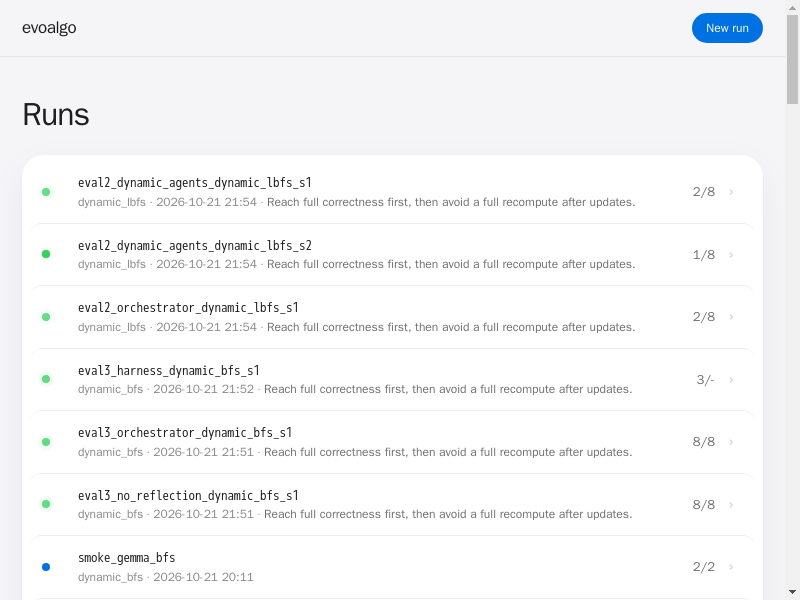
\includegraphics[width=\textwidth]{../campaign/ui_check/01_runs.png}
\caption{The run list. Each row shows the run id, the pack, the last update
time, the research goal, the generation counter, a fitness sparkline, and the
best work ratio. The \textbf{New run} button starts a launch.}
\label{fig:ud-runs}
\end{figure}

\begin{figure}[H]
\centering
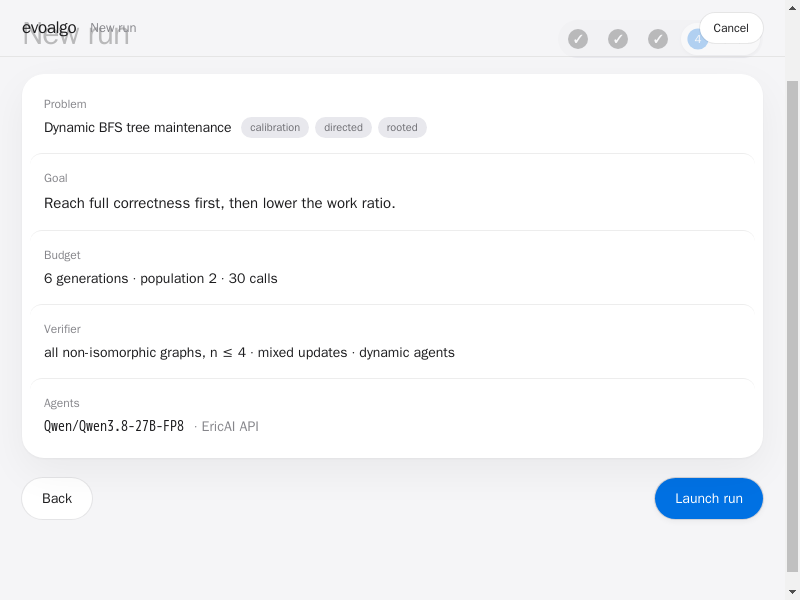
\includegraphics[width=\textwidth]{../campaign/ui_check/03_review.png}
\caption{The Review step of the New Run form for a dynamic BFS run: the chosen
pack and its tags, the goal, the budget (6 generations, population 2, 30
calls), the verifier (all non-isomorphic graphs, $n \le 4$, mixed updates,
dynamic agents), and the agent (Qwen3.8-27B-FP8 over the EricAI API). The
stepper at the top marks the first three steps done.}
\label{fig:ud-review}
\end{figure}

\subsection{Monitor a run live}
\label{sec:ud-monitor}

The live view (Figure~\ref{fig:ud-live}) streams the run's event log over a
websocket and renders, from the top down: a status line (generation, best
candidate, work ratio, and the active hint if any); four KPI tiles (best
fitness, best work ratio, pass rate, model calls) each with a sparkline; a
work-ratio chart (best and mean per generation); a lineage chart (candidates
and their parents); the event log (every agent call, verification, commit, and
cull with its duration); the population table (candidate, parent, role,
fitness, work ratio); the failure-patterns panel (failures grouped by kind and
by the size of the first failing graph); and, when dynamic agents are on, the
specialist-agents panel.

\begin{enumerate}
  \item Open a running run from the list.
  \item Watch the KPI tiles and the event log update as generations commit.
  \item Switch to the failure-patterns panel to see why candidates are failing.
\end{enumerate}

\emph{Expected result:} the view tracks the run in real time; a committing
generation updates the best fitness and work ratio and appends events.
\emph{Recovery:} if the view shows the run as \emph{offline} or
\emph{interrupted}, the engine process is gone; Section~\ref{sec:ud-trouble}
covers resuming. The command-line equivalent is \texttt{evoalgo status
<run\_dir>}.

\begin{figure}[H]
\centering
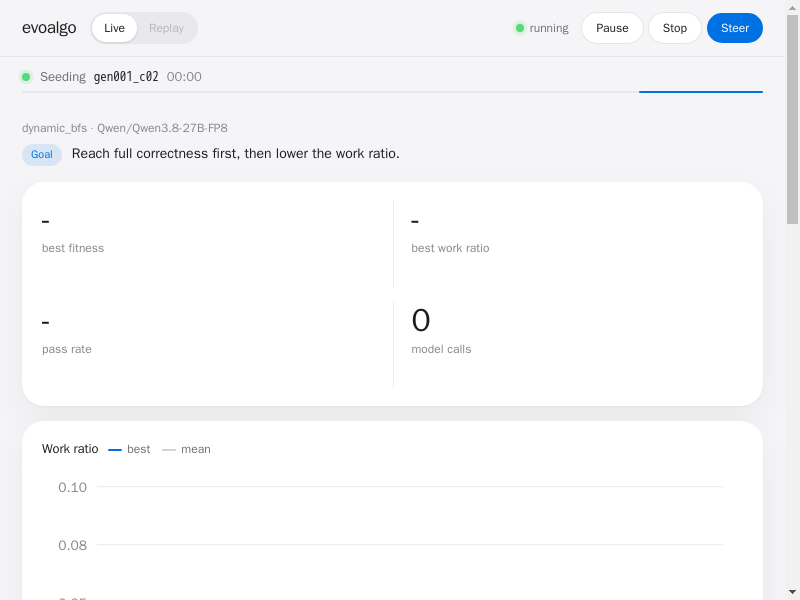
\includegraphics[width=\textwidth]{../campaign/ui_check/04_live.png}
\caption{The live view at the start of a run: the status line reads
\emph{Seeding gen001\_c02}, the four KPI tiles are empty (no committed
generation yet), and the work-ratio chart is waiting for data. The Live/Replay
toggle, the running status, and the Pause, Stop, and Steer controls are at the
top.}
\label{fig:ud-live}
\end{figure}

\subsection{Steer a running run}
\label{sec:ud-steer}

Steering changes the search without restarting it. The controls are the
\textbf{Pause}, \textbf{Stop}, and \textbf{Steer} buttons at the top of the run
page, and the Steer panel (Figure~\ref{fig:ud-done} shows it open over a
finished run).

\begin{enumerate}
  \item Click \textbf{Steer}. The panel offers a \emph{Hint} field (free text,
  up to 2000 characters), a \emph{Call budget} field, and a \emph{Population}
  field.
  \item Enter a hint, a new budget, or a new population, and click
  \textbf{Apply at next generation}. A hint is carried into every subsequent
  agent call; an empty hint clears it.
  \item To pause, click \textbf{Pause}; the engine applies it before the next
  model call and the status moves to \emph{paused}. Click \textbf{Resume} to
  continue. \textbf{Stop} ends the run at the next generation boundary,
  committing whatever was produced.
\end{enumerate}

\emph{Expected result:} each command is acknowledged by the engine with a
\texttt{control\_ack} event, which appears in the event log; the hint is shown
in the status line of the generation it is applied at. \emph{Recovery:} a
command sent to an ended run is refused (\texttt{control\_reject}); the event
log shows the refusal and the run state. The command-line equivalent is
\texttt{evoalgo control <run\_dir> hint "text"}, \texttt{... set
population\_size 4}, \texttt{... pause}, \texttt{... resume}, or \texttt{...
stop}.

\subsection{Replay the generation history}
\label{sec:ud-replay}

\begin{enumerate}
  \item On a finished run, click the \textbf{Replay} toggle.
  \item Drag the generation scrubber to a generation, or press the play button
  to step through generations one by one.
  \item The KPIs, charts, population, and failure patterns re-render for the
  scrubbed generation.
\end{enumerate}

\emph{Expected result:} the view shows the committed state at the chosen
generation, including any hint that was applied there. \emph{Recovery:} replay
is read-only over committed checkpoints; if a generation is missing, the run
was stopped before committing it (see
Section~\ref{sec:ud-trouble}). The command-line equivalent is
\texttt{evoalgo export <run\_dir>}, which writes the per-candidate history to
CSV.

\subsection{Inspect a candidate}
\label{sec:ud-inspect}

\begin{enumerate}
  \item In the population table, the lineage chart, or the failure-patterns
  panel, click a candidate.
  \item The drawer opens (Figure~\ref{fig:ud-faildrawer}) showing the
  candidate's metrics (fitness, work ratio, tests passed over total, parent),
  its failing case when it failed (the operation, the graph size, and the
  expected versus actual value), its reflection when one was written, and its
  full source code.
\end{enumerate}

\emph{Expected result:} the drawer shows the code and, for a failure, the first
failing case that the verifier located. \emph{Recovery:} the drawer loads the
candidate file from the run directory; if the file is absent the candidate was
culled and its code is no longer kept. The command-line equivalent is to open
\texttt{<run\_dir>/candidates/<id>.py}.

\begin{figure}[H]
\centering
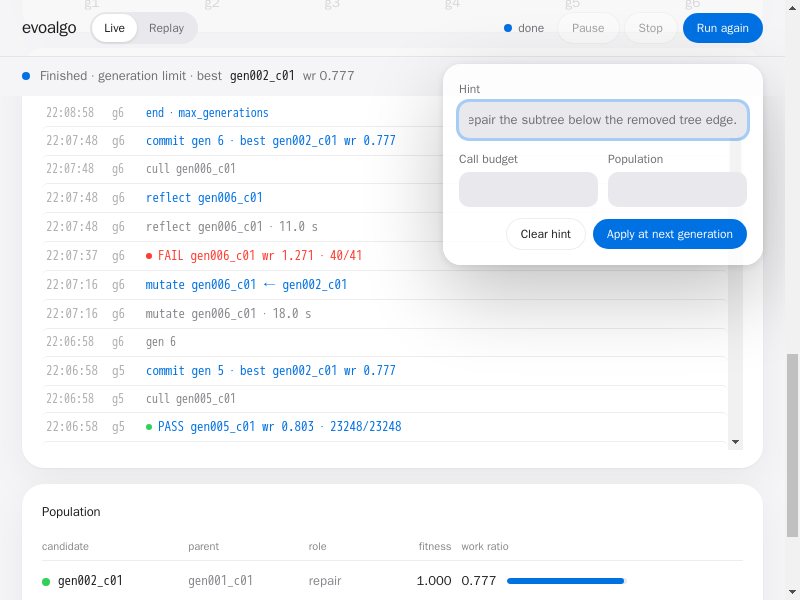
\includegraphics[width=\textwidth]{../campaign/ui_check/06_done.png}
\caption{A finished run with the Steer panel open. The status line reads
\emph{Finished $\cdot$ generation limit $\cdot$ best gen002\_c01 wr 0.777};
the event log shows the generation 6 commits, culls, and a FAIL with its first
failing case; the population table lists the best candidate. The Steer panel
offers a hint, a call budget, and a population, with \emph{Clear hint} and
\emph{Apply at next generation}.}
\label{fig:ud-done}
\end{figure}

\begin{figure}[H]
\centering
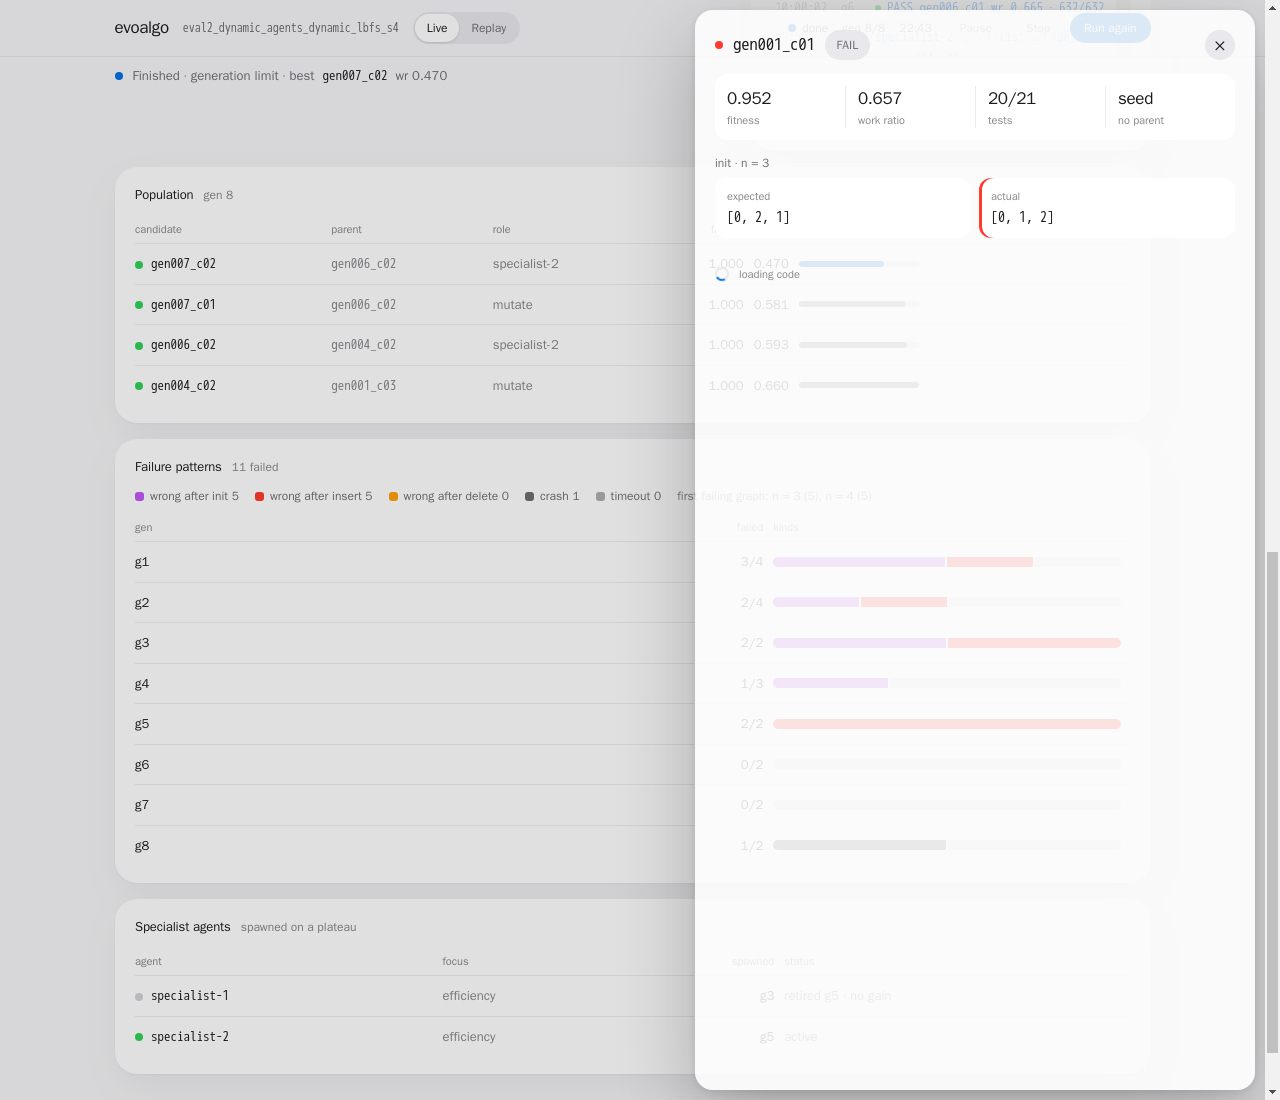
\includegraphics[width=\textwidth]{../campaign/ui_check/09_failure_drawer.png}
\caption{The candidate drawer over a finished dynamic LBFS run. The header shows
the candidate id and its FAIL state; the metrics row shows fitness, work ratio,
tests (20/21), and the role (seed, no parent). The failing case shows the
operation (\texttt{init} at $n = 3$) with the expected and actual values.
Behind the drawer are the population, the failure-patterns panel (11 failed,
grouped by kind and by first-failing size), and the specialist-agents panel
(specialist-1 retired, specialist-2 active).}
\label{fig:ud-faildrawer}
\end{figure}

\subsection{Command-line-only operation}
\label{sec:ud-cli}

The full command set, with the equivalent of every web action:

\begin{enumerate}
  \item \textbf{Configure and start.}
  \texttt{evoalgo configure --problem dynamic\_bfs} with \texttt{-o
  config.yaml}, then \texttt{evoalgo start config.yaml --run-id myrun}.
  \item \textbf{Status.} \texttt{evoalgo status runs/myrun} (add
  \texttt{--json} for a machine-readable summary including the final grade and
  the best candidate path).
  \item \textbf{Control.} \texttt{evoalgo control runs/myrun hint "text"},
  \texttt{... set model\_call\_budget 100}, \texttt{... pause},
  \texttt{... resume}, \texttt{... stop}.
  \item \textbf{Resume.} \texttt{evoalgo resume runs/myrun} reloads the last
  committed generation and continues; a harness workspace is refused here and
  must be continued with \texttt{evoalgo check}.
  \item \textbf{Export.} \texttt{evoalgo export runs/myrun} writes
  \texttt{results/run\_summary.json} and
  \texttt{results/efficiency\_report.csv}.
  \item \textbf{History.} \texttt{evoalgo history} lists previous runs with
  generation, best fitness, best work ratio, pass count, and problem.
\end{enumerate}

\emph{Expected result:} each command prints a short summary; \texttt{start}
prints the final run summary. \emph{Recovery:} a refused or invalid command
prints the reason and exits non-zero without starting a run.

\subsection{The coding-agent harness}
\label{sec:ud-harness}

The harness exposes the same verifier to an external coding agent. The agent
edits one file; the tool grades it and records each grade as a run.

\begin{enumerate}
  \item \textbf{Initialize a workspace.} \texttt{evoalgo init dynamic\_bfs}
  (optionally a target directory, \texttt{--goal}, \texttt{--harness}, and
  \texttt{--max-checks}). This creates \texttt{program.md} (the instructions),
  \texttt{candidate.py} (a starter), and \texttt{results.tsv}, and starts a
  live run shown in the interface.
  \item \textbf{Let the agent work.} The agent edits \texttt{candidate.py} and
  runs \texttt{evoalgo check} (default level \texttt{search}, $n \le 4$), or
  \texttt{check --level examples} ($n \le 3$) for a cheaper check, or
  \texttt{check --level full} ($n \le 5$). The command prints a JSON report and
  exits 0 on PASS, 3 on FAIL, 2 on error.
  \item \textbf{Final grade.} When the agent is satisfied it runs
  \texttt{evoalgo check --final}, the tool's independent re-grade of the kept
  candidate on the full bound. This is the one final grade; repeating it is
  refused.
  \item \textbf{Finish.} \texttt{evoalgo finish} closes the workspace run.
\end{enumerate}

\emph{Expected result:} each check is logged to \texttt{results.tsv} and to the
run folder; the final verdict is the \texttt{--final} re-grade.
\emph{Recovery:} grading a file other than \texttt{candidate.py}, exceeding
\texttt{max\_checks}, or repeating \texttt{--final} is refused with a named
reason. The final grade takes about 10 minutes on BFS/DFS; give the command at
least 15 minutes (Section~\ref{sec:ud-trouble}).

Each \texttt{check} prints a JSON report the agent reads: the verdict
(\texttt{PASS} or \texttt{FAIL}), the grade level, the tests passed over total,
the work ratio, and, on a failure, the first failing case. The tool also stores
a SHA-256 snapshot of the graded \texttt{candidate.py}; if the file is edited
after a grade, the report marks that snapshot as not intact, so a later
\texttt{--final} is a re-grade of the file as it was when it was kept, not of a
file the agent has since changed. The levels are ordered by cost:
\texttt{examples} ($n \le 3$) is a few seconds, \texttt{search} ($n \le 4$) is
the default and also a few seconds, and \texttt{full} ($n \le 5$) is the
minutes-long final grade. An agent typically iterates on \texttt{search} and
finishes with one \texttt{--final}.

The same harness is packaged as an Agent Skill \citep{agentskills}. Inside the
repository it is picked up automatically from \texttt{.agents/skills} and
\texttt{.claude/skills}; elsewhere it is installed with
\texttt{evoalgo skill --install}, which copies it to the home directory's
\texttt{.agents/skills} and \texttt{.claude/skills} (or \texttt{--project}
into the current repository). Once installed, a coding agent can be asked, for
example, to use the evoalgo skill to find a dynamic BFS algorithm for the
\texttt{dynamic\_bfs} pack, and each session appears as a run in
\texttt{evoalgo ui}.

\subsection{The verifier self-test as a user}
\label{sec:ud-verify}

The self-test checks the verifier itself, not a candidate: it runs the
known-good references (which must pass), every seeded fault (which must be
rejected), and the equivalent controls (which must be accepted), over the
bounded universe.

\begin{enumerate}
  \item Run \texttt{evoalgo verify --problem dynamic\_bfs --n-max 3} (a small
  bound for a quick check; the default for the corpus problems is 5).
  \item Read the summary table and the final line.
\end{enumerate}

The command was run at $n \le 3$ and its final lines are:

\begin{lstlisting}[language=bash, basicstyle=\ttfamily\small]
  Zero-false-negative (n<=3): 14/14 real faults rejected -> PASS
  Known-good accepted: PASS
  Equivalent controls accepted: PASS

  Verifier self-test: ALL PASS
\end{lstlisting}

\emph{What ALL PASS means:} every reference and control was accepted and every
seeded fault was rejected at the stated bound, so the verifier is not
permissive (it rejects wrong candidates) and not over-strict (it accepts valid
variants). It is a bounded check, not a proof. The full $n \le 5$ self-test for
BFS, DFS, and LBFS is reported in Chapter~\ref{ch:testing}; the command-line
\texttt{--relabels 2} flag reproduces the full documented universe.

\section{The three complex features, from the user's view}
\label{sec:ud-features}

The three registered contributions are used through the workflows above; this
section states, for each, the user goal, the preconditions, the steps, the
visible result, and the failure recovery, without repeating the step lists.

\subsection{Feature C1: the research tool interface}

\emph{Goal:} launch, monitor, and replay a multi-generation run end to end from
one place. \emph{Preconditions:} an installed package with the \texttt{ui}
extra, a run directory root, and (for an API run) a model key in the named
environment variable. \emph{Steps:} launch from the New Run page
(Section~\ref{sec:ud-launch}), monitor live (Section~\ref{sec:ud-monitor}),
steer (Section~\ref{sec:ud-steer}), and replay (Section~\ref{sec:ud-replay}).
\emph{Visible result:} the live view with KPIs, charts, population, failure
patterns, and specialists; the replay scrubber; and the candidate drawer.
\emph{Failure recovery:} a refused launch names its blocking field; an
interrupted run is resumed (Section~\ref{sec:ud-trouble}); a missing token is
recovered from the printed link or \texttt{runs/.ui-link}.

\subsection{Feature C2: the isomorphism-aware verifier}

\emph{Goal:} trust a candidate's correctness and measure its efficiency.
\emph{Preconditions:} a Linux host with user namespaces (or an explicit
\texttt{EVOALGO\_SANDBOX=none}), and the committed \texttt{nauty} data.
\emph{Steps:} the verifier runs automatically on every candidate during a run
and on the best candidates at the end; the user-facing action is the self-test,
\texttt{evoalgo verify} (Section~\ref{sec:ud-verify}). \emph{Visible result:}
each candidate's state (PASS, FAIL, or CRASH), its fitness, its work ratio, and
its first failing case in the drawer; the self-test's \texttt{ALL PASS} line.
\emph{Failure recovery:} a CRASH or TIMEOUT is a located failure, not a silent
pass; a sandbox that cannot start fails closed with a named error
(Section~\ref{sec:ud-trouble}).

\subsection{Feature C3: cooperative and dynamic agents}

\emph{Goal:} let specialized agents repair candidates, and spawn new
specialists when the search plateaus, without human intervention.
\emph{Preconditions:} a model endpoint (or mock), and, for dynamic agents, the
\emph{spawn a specialist agent when the search plateaus} toggle on the New Run
page (or \texttt{dynamic\_agents: true} in the config). \emph{Steps:} launch
with the toggle; the orchestrator runs the generator, reflector, and repairer
roles, and on a plateau spawns a specialist whose focus is written from the
plateau, retires it after its budget or a window without gain.
\emph{Visible result:} the specialist-agents panel (spawned, focus, status) and
specialist-labelled candidates in the population. \emph{Failure recovery:} a
run with no plateau never spawns a specialist, which is correct; a specialist
that does not improve the search is retired and the run continues.

\section{Results and files}
\label{sec:ud-results}

Every run is a directory under the workdir (default \texttt{runs/}). For a
finished run the directory contains, and the user reads, the following:

\begin{itemize}
  \item \texttt{config.yaml} : the validated configuration actually used.
  \item \texttt{events.jsonl} : the event log, one JSON object per line, with
  contiguous sequence numbers. It is the source for the live view, the replay,
  and the status command.
  \item \texttt{generation\_NNNN.json} : one checkpoint per committed
  generation, holding that generation's candidates, fitness, work ratios, and
  parents. \texttt{COMMITTED} holds the highest committed generation number.
  \item \texttt{candidates/} : the source code of each candidate, one
  \texttt{<id>.py} per candidate.
  \item \texttt{reflections/} : the reflector's failure analysis, one
  \texttt{<id>.md} per reflected candidate.
  \item \texttt{prompt\_logs/} : one JSON file per agent call (role, model,
  duration, token usage, tool calls), for auditing what the model was asked.
  \item \texttt{results/run\_summary.json} and
  \texttt{results/efficiency\_report.csv} : written by \texttt{evoalgo export};
  the summary holds the run id, total generations and candidates, best fitness,
  best candidate id, best work ratio, and pass count; the CSV holds one row per
  candidate with generation, fitness, work ratio, state, timeout flag, and
  tests passed over total.
  \item \texttt{dashboard/} : an HTML snapshot per \texttt{dashboard\_interval}
  generations, for a static view without the live server.
\end{itemize}

The mock run's \texttt{run\_summary.json} was:

\begin{lstlisting}[language=bash, basicstyle=\ttfamily\small]
{
  "run_id": "smoke_mock",
  "total_generations": 1,
  "total_candidates": 2,
  "best_fitness": 1.0,
  "best_candidate_id": "gen001_c01",
  "best_work_ratio": 0.4299706170421156,
  "passing": 2
}
\end{lstlisting}

Reading the numbers: \emph{fitness} is 1.0 for a candidate that passed its
grade and below that otherwise, so the best fitness tells you whether a correct
candidate was found at all. The \emph{work ratio} is the candidate's time over
the offline recomputation baseline on the graded graphs; below 1 means the
candidate is cheaper than recomputing, and it is the number the search optimizes
after correctness. A run uses two grades (Refinement R3 in
Chapter~\ref{ch:requirements}): every candidate is graded during the run on the
small search bound ($n \le 4$ by default), and the best passing candidates are
graded again at the end on the full bound ($n \le 5$). The search grade is fast
and is what the KPIs track live; the final grade is the one that determines the
run's verdict, and a candidate can pass the search grade yet fail the final
grade on a fault that only appears at $n = 5$. The \texttt{final\_graded} event
in \texttt{events.jsonl} records that verdict, and the \texttt{--json} form of
\texttt{status} surfaces it together with the best candidate path.

To export a run, run \texttt{evoalgo export <run\_dir>}; it prints
\texttt{Exported to <run\_dir>/results/} and the two files it wrote. The
\texttt{--json} form of \texttt{status} adds the final grade and the best
candidate path, which is convenient for a supervisor reviewing a run
programmatically.

\section{Troubleshooting, limitations, and FAQ}
\label{sec:ud-trouble}

Table~\ref{tab:ud-trouble} lists the common failures, each verified against the
source or a run. The \emph{Resolution} column gives the safe fix.

\begin{scriptsize}
\setlength{\tabcolsep}{4pt}
\begin{longtable}{@{}p{0.26\textwidth}p{0.34\textwidth}p{0.34\textwidth}@{}}
\caption{Troubleshooting guide (verified cases).}\label{tab:ud-trouble}\\
\toprule
\textbf{Symptom} & \textbf{Cause / diagnosis} & \textbf{Resolution and recovery} \\
\midrule
\endfirsthead
\toprule
\textbf{Symptom} & \textbf{Cause / diagnosis} & \textbf{Resolution and recovery} \\
\midrule
\endhead
\bottomrule
\endfoot
\texttt{the sandbox needs Linux user namespaces (unshare)}; the run refuses to start. & The host has no unprivileged user namespaces, or \texttt{unshare} is missing; the sandbox fails closed. & Enable unprivileged user namespaces on the host. For debugging only, set \texttt{EVOALGO\_SANDBOX=none}, which runs candidates unconfined at the user's own risk. \\
\addlinespace[2pt]
\texttt{API key not found: export ERICAI\_ACCESS\_TOKEN}. & The \texttt{api} backend could not read the key variable. & Export the named variable before starting (\texttt{export ERICAI\_ACCESS\_TOKEN=...}); only the name is stored, the value is read at call time. \\
\addlinespace[2pt]
A run stalls or fails with an auth error on EricAI. & The EricAI token is short-lived and expired. & The token is re-read from \texttt{\textasciitilde/.ericai\_token\_env} on every call and refreshed automatically about 10 minutes before expiry; if the automatic refresh fails, run \texttt{ericai --ericsson-access-token} interactively once. \\
\addlinespace[2pt]
\texttt{missing or wrong access token: open the link printed by evoalgo ui}. & The browser has no valid token cookie. & Open the printed link (or the one in \texttt{runs/.ui-link}); it sets an HttpOnly cookie. The link is single-use per server and dies when the server stops. \\
\addlinespace[2pt]
A run is shown as \emph{interrupted} in the UI. & The engine process exited (crash, host reboot, or a stop). & Run \texttt{evoalgo resume <run\_dir>}; it discards any incomplete generation and continues from the last committed checkpoint. \\
\addlinespace[2pt]
A candidate is \texttt{TIMEOUT}, \texttt{CRASH}, or \texttt{FAIL}. & The candidate hung, raised an exception, or violated the invariant, respectively. & All three are failures, never passes. The drawer shows the located failing case (graph, operation, expected vs actual); use it to steer with a hint. \\
\addlinespace[2pt]
\texttt{evoalgo check --final} appears to hang or is killed by a shell timeout. & The final grade on the full bound takes about 10 minutes for BFS/DFS. & Give the command at least 15 minutes; the workspace brief and the skill now state this. The grade is bounded and will finish. \\
\addlinespace[2pt]
The run stops early with a budget stop reason. & The \texttt{model\_call\_budget} was used. & Raise the budget on the New Run page or via \texttt{evoalgo control <run\_dir> set model\_call\_budget N}, then resume. \\
\addlinespace[2pt]
\texttt{evoalgo ui} fails to bind the port. & Port 8765 is already in use. & Start with \texttt{--port <other>}; the access link is printed for that port. \\
\addlinespace[2pt]
\texttt{check budget used up (N checks); run evoalgo check --final, then evoalgo finish}. & \texttt{max\_checks} was reached. & Run the one final grade, then \texttt{evoalgo finish}; further checks are refused by design. \\
\addlinespace[2pt]
A launch is blocked with \texttt{enlcode not found on this machine}. & The harness agent binary is not on the path. & Install the harness or choose an API endpoint instead; the New Run page names the missing prerequisite. \\
\addlinespace[2pt]
\texttt{evoalgo ui} prints \texttt{The UI needs the 'ui' extra}. & The package was installed without the \texttt{ui} extra. & Reinstall with \texttt{pip install -e '.[ui]'} (or \texttt{'.[api,ui]'}). \\
\bottomrule
\end{longtable}
\end{scriptsize}

\subsection{Limitations}

These are stated plainly so a user does not over-read a result.

\begin{itemize}
  \item \textbf{Bounded verification is not a proof.} A candidate that passes
  has no counterexample within the stated bound ($n \le 5$ by default); a fault
  that only appears on a larger graph is not caught. The word ``proof'' is
  reserved for a mathematical or formal proof, which is out of scope.
  \item \textbf{The bound is small.} The exhaustive universe is $n \le 5$;
  beyond it the verifier uses seeded random sampling, so coverage past the
  bound is sampled, not exhaustive.
  \item \textbf{Model sampling is not seeded.} The test universe and parent
  selection are reproducible, but the language model's sampling is not; two
  runs with the same configuration do not produce identical fitness
  trajectories.
  \item \textbf{Linux only for the jail.} The sandbox requires Linux user
  namespaces; on other platforms it fails closed unless explicitly disabled.
  \item \textbf{Single user, loopback.} The interface binds to 127.0.0.1 and is
  intended for one researcher on one host; there is no multi-user service and
  no enforced read-only role.
\end{itemize}

\subsection{Frequently asked questions}

\begin{description}
  \item[Do I need to install nauty or graph data?] No. The representative
  digraph files are committed in the repository; the tool only reads them.
  \item[Can I run a search without a model key?] Yes. Set
  \texttt{provider: mock}; the mock writes a known-good recompute candidate, so
  a small run finishes in seconds and exercises the whole pipeline. It is for
  trials and demos, not for discovery.
  \item[What does a work ratio below 1 mean?] The candidate is cheaper than
  recomputing the result from scratch on the graded graphs; it is the efficiency
  signal the search optimizes after correctness.
  \item[Is a passing candidate proven correct?] No. It has no counterexample
  within the stated bound ($n \le 5$ by default). That is bounded exhaustive
  verification, not a proof (Refinement R3).
  \item[Can I run two runs at once?] Yes; each run is its own directory and the
  sandbox gives every candidate its own namespace and resource budget. The web
  interface lists both and you switch between them.
  \item[Where do my runs go, and how do I remove them?] Under the workdir
  (default \texttt{runs/}); delete the run directory to remove it, as described
  in Section~\ref{sec:ud-security}.
\end{description}

\section{Security, privacy, backup, and data removal}
\label{sec:ud-security}

\subsection{What is sent to the model provider}

When the \texttt{api} backend is used, each agent call sends the problem brief
(the pack's \texttt{brief.md}), the candidate code being generated or repaired,
the first failing case when repairing, and any active hint. No user files, no
host configuration, and no credentials are sent. The API key is read from the
environment at call time and is never written to a config, a log, or a
prompt; the configuration stores only the variable \emph{name}
(\texttt{api\_key\_env}). Auth errors are logged with the status and the
provider's error code only, not the response body, so a key echoed by a
provider is not captured in the (committed) call log.

\subsection{Sandbox guarantees, in user terms}

Candidate code is model-written and untrusted. It runs inside a Linux
namespace jail: no network (the network namespace is down), no home directory
or token files (the home, shared, and temp trees are hidden behind an empty
tmpfs and the interpreter's import paths are bound back read-only), its own pid
namespace, and its own IPC namespace so shared memory does not outlive the
candidate. Resource limits are enforced before any candidate code runs: 4 GB of
address space, CPU time equal to the wall-clock timeout plus 5 seconds, 4
processes, 16 MB per file, 64 open files, 256 MB of result output, and 64 KB of
stderr. A candidate that tries to read a secret, reach the network, or exhaust
the host is blocked and reported as a failure, not a pass. Where the jail is
unavailable the sandbox refuses to run unless \texttt{EVOALGO\_SANDBOX=none} is
set, which removes these guarantees and is for debugging only.

\subsection{Secrets handling}

The only secret the tool touches is the model API key, and it is handled by
name: the config and the New Run page store and show the variable name and
whether a value is present, never the value. The EricAI token file
(\texttt{\textasciitilde/.ericai\_token\_env}) is created with mode 600 and
refreshed under a file lock so parallel runs refresh once between them. The UI
access token is generated per server, printed once (or written to
\texttt{runs/.ui-link} with mode 600 when output is redirected), and deleted
when the server stops.

\subsection{Backup and data removal}

There is no database and no remote store: a run is fully described by its
directory under the workdir. To back up a run, copy its directory; to remove
it, delete the directory. Deleting a run directory removes its candidates,
reflections, prompt logs, checkpoints, event log, and exported results
together, and the run disappears from the interface list and from
\texttt{evoalgo history}. The \texttt{runs/.ui-link} file is removed
automatically when the server stops. Nothing is written outside the workdir
except the EricAI token file in the home directory and the installed Agent
Skill in \texttt{\textasciitilde/.agents/skills} or
\texttt{\textasciitilde/.claude/skills} (removed by deleting those directories).
